\documentclass[journal,12pt,twocolumn]{IEEEtran}
\usepackage{cite}
\usepackage{amsmath,amssymb,amsfonts,amsthm}
\usepackage{algorithmic}
\usepackage{graphicx}
\usepackage{textcomp}
\usepackage{xcolor}
\usepackage{txfonts}
\usepackage{listings}
\usepackage{enumitem}
\usepackage{mathtools}
\usepackage{gensymb}
\usepackage{comment}
\usepackage[breaklinks=true]{hyperref}
\usepackage{tkz-euclide} 
\usepackage{circuitikz}
\usepackage{pgfplots}                            
\usepackage[latin1]{inputenc}                                
\usepackage{color}                                            
\usepackage{array}                                            
\usepackage{longtable}                                       
\usepackage{calc}                                             
\usepackage{multirow}                                         
\usepackage{hhline}                                           
\usepackage{ifthen}                                           
\usepackage{lscape}

\newtheorem{theorem}{Theorem}[section]
\newtheorem{problem}{Problem}
\newtheorem{proposition}{Proposition}[section]
\newtheorem{lemma}{Lemma}[section]
\newtheorem{corollary}[theorem]{Corollary}
\newtheorem{example}{Example}[section]
\newtheorem{definition}[problem]{Definition}
\newcommand{\BEQA}{\begin{eqnarray}}
\newcommand{\EEQA}{\end{eqnarray}}
\newcommand{\define}{\stackrel{\triangle}{=}}
\theoremstyle{remark}
\newtheorem{rem}{Remark}

\usepackage{pgfplots}
\pgfplotsset{width=7cm,compat=1.16}

\begin{document}

\bibliographystyle{IEEEtran}
\vspace{3cm}

\title{NCERT Physics 12.7. Q20}
\author{EE23BTECH11204- Ashley Ann Benoy$^{*}$% <-this % stops a space
}
\maketitle
\newpage
\bigskip

\renewcommand{\thefigure}{\theenumi}
\renewcommand{\thetable}{\theenumi}

\bibliographystyle{IEEEtran}

\textbf{Question}

A series LCR circuit with 
\(L = 0.12 \, \text{H}\),
\(C = 480 \times 10^{-9} \, \text{F}\), 
\(R=23 \, \Omega\)
is connected to a 230 V variable frequency supply.

(a) What is the source frequency for which current amplitude is maximum? Obtain this maximum value.

(b) What is the source frequency for which the average power absorbed by the circuit is maximum? Obtain the value of this maximum power.

(c) For which frequencies of the source is the power transferred to the circuit half the power at resonant frequency? What is the current amplitude at these frequencies?

(d) What is the Q-factor of the given circuit?

\textbf{Solution:}
Given parameters are:
\setcounter{table}{0} % Set the table number to 1
\textbf{
\begin{table}[htbp]
\centering
\caption{Given Data}
\label{tab:data}
\begin{tabular}{|c|c|c|}
\hline
\textbf{Symbol} & \textbf{Value} & \textbf{Parameter} \\
\hline
\(L\) & \(0.12 \, \text{H}\) & Inductance \\
\(C\) & \(480 \, \text{nF}\) & Capacitance \\
\(R\) & \(23 \, \Omega\) & Resistance \\
\(V\) & \(230 \, \text{V}\) & Supply voltage \\
\hline
\end{tabular}
\end{table}
}



% goes into figs

\begin{figure}[htb]
    \centering
    \begin{circuitikz} 
        \draw (0,0)
        to[sinusoidal voltage source, v=$V$] (0,2) % Voltage source
        to[R, l=$R$] (2,2) % Resistor
        to[L, l=$sL$] (4,2) % Inductor
        to[C, l=$\frac{1}{sC}$] (4,0); % Capacitor
        \draw (4,2) to[short, -o] (5,2) node[right] {Terminal}; % Terminal label
        \draw (0,0) to[short, -o] (5,0) node[right] {Terminal}; % Terminal label
    \end{circuitikz}
    \caption{Circuit diagram with sinusoidal voltage source, resistor, inductor, and capacitor.}
    \label{fig:circuit}
\end{figure}


The impedance of the above circuit is given as:
\begin{align}
  H(s) &= \dfrac{V(s)}{I(s)}\\
     H(s) &= R + sL + \dfrac{1}{sC}\\
     \implies H(j\omega) &= R + j\omega L + \dfrac{1}{j\omega C}\\
     \implies \lvert H(j\omega) \rvert &= \sqrt{R^2 + \left(\omega L - \dfrac{1}{\omega C}\right)^2}
\end{align}

%part A
 At resonance, the circuit becomes purely resistive. The reactances of capacitor and inductor cancel out as follows:
\begin{align}
    Ls + \frac{1}{sC} &= 0 \\
    \implies s &= j\frac{1}{\sqrt{LC}} = j\omega
\end{align}
The current (\(I\)) is given by Ohm's Law as:
\begin{align}
    I &= \frac{V}{Z} = \frac{V}{R + j(\omega L - \frac{1}{\omega C})}
\end{align}

Substitute the expression for \(Z\) into the current equation:
\begin{align}
    I &= \frac{V}{R + j(\omega L - \frac{1}{\omega C})} \\
    &= \frac{V(R - j\omega L + \frac{1}{\omega C})}{(R + j\omega L - \frac{1}{\omega C})(R - j\omega L + \frac{1}{\omega C})}
\end{align}

To simplify this expression, you can multiply the numerator and denominator by the conjugate of the denominator:
\begin{align}
    I &= \frac{V(R - j\omega L + \frac{1}{\omega C})}{(R + j\omega L - \frac{1}{\omega C})(R - j\omega L + \frac{1}{\omega C})} \\
    &= \frac{(R + j\omega L - \frac{1}{\omega C})(R - j\omega L + \frac{1}{\omega C})}{(R^2 + (\omega L - \frac{1}{\omega C})^2)}
\end{align}

Now, combine like terms and take the magnitude of the expression to get the amplitude of the current:
\begin{align}
    |I| &= \frac{V}{\sqrt{(R - \frac{1}{\omega C})^2 + (\omega L)^2}}
\end{align}

\begin{align}
    I &= \frac{V}{\sqrt{R^2 + (\omega L - \frac{1}{\omega C})^2}} \angle -\tan^{-1}\left(\frac{\omega L - \frac{1}{\omega C}}{R}\right)
\end{align}

The source frequency for maximum current amplitude is given by:
\begin{align}
    \omega_{\text{max}} &= \frac{1}{\sqrt{LC}}\label{eq:omega_max}
\end{align}

%part B
The source frequency for which the average power absorbed by the circuit is maximum is the same as the resonance frequency. 
\begin{align}
    I_{\text{max}} &= \frac{V}{Z_{\text{total}}} = \frac{V}{R}
\end{align}

At resonance, \(Z_{\text{total}} = R\), so \(I_{\text{max}} = \frac{V}{R}\).
\begin{align}
    P_{\text{avg}} &= \frac{1}{2} I_{\text{max}}^2 R
\end{align}

Substitute \(I_{\text{max}} = \frac{V}{R}\) into the expression for \(P_{\text{avg}}\):
\begin{align}
    P_{\text{avg}} &= \frac{1}{2} \left(\frac{V}{R}\right)^2 R
\end{align}
\begin{align}
    P_{\text{avg}} &= \frac{1}{2} \frac{V^2}{R}
    \label{eq:9}
\end{align}

%part C
The power in the circuit is $P_{\text{max}} = i_{\text{max}}^2 R$. At the half frequencies, the power of the circuit is $P = \frac{P_{\text{max}}}{2} = \frac{i_{\text{max}}^2 R}{2} = \left(\frac{i_{\text{max}}^2}{\sqrt{2}}\right)^2 R$. This means that the current in the circuit at half power frequencies is $\frac{i_{\text{max}}}{\sqrt{2}}$. Then, $V = \frac{i_{\text{max}}}{\sqrt{2}} Z$.

Substitute the value of $i_{\text{max}}$ 
\begin{align}
    V &= \left(\frac{V}{R}\right)^{\frac{2}{\sqrt{2}}} Z \quad \Rightarrow \quad 2^{\frac{1}{\sqrt{2}}} R = Z \quad \Rightarrow \quad 2R^2 = Z^2
\end{align}

However, $Z^2 = R^2 + \left(2\pi f L - \frac{1}{2\pi f C}\right)^2$. Therefore,
\begin{align}
    2R^2 &= R^2 + \left(2\pi f L - \frac{1}{2\pi f C}\right)^2 \\
    \Rightarrow \quad R^2 &= \left(2\pi f L - \frac{1}{2\pi f C}\right)^2
\end{align}

\begin{align}
    \Rightarrow \quad R &= \pm \left(2\pi f L - \frac{1}{2\pi f C}\right)
\end{align}

This proves that there are two values of half power frequencies. Therefore,
\begin{align}
    R &= 2\pi f_1 L - \frac{1}{2\pi f_1 C} \quad \text{or} \quad R = \frac{1}{2\pi f_2 C} - 2\pi f_2 L.
\end{align}

\begin{align}
    R &= 4\pi^2 f_1^2 LC - \frac{1}{2\pi f_1 C} \\
    \Rightarrow \quad 2\pi f_1 C R &= 4\pi^2 f_1^2 LC - 1 \quad \ldots \,
\end{align}

And
\begin{align}
    R &= \frac{1 - 4\pi^2 f_2^2 LC}{2\pi f_2 C} \\
    \Rightarrow \quad 2\pi f_2 C R &= 1 - 4\pi^2 f_2^2 LC \quad \ldots \,
\end{align}

Add (iii) and (iv):
\begin{align}
    2\pi f_1 C R + 2\pi f_2 C R &= 4\pi^2 f_1^2 LC - 1 + 1 - 4\pi^2 f_2^2 LC
\end{align}

\begin{align}
    \Rightarrow (f_1 + f_2) R &= 2\pi (f_1^2 - f_2^2) L \\
    \Rightarrow (f_1 + f_2) R &= 2\pi (f_1 + f_2)(f_1 - f_2) L \quad \ldots \, \\
    \Rightarrow (f_1 - f_2) &= \frac{R}{2\pi L}.
\end{align}

The difference in the half power frequencies, i.e., $(f_1 - f_2)$, is called bandwidth.

Additionally, in terms of angular frequency \(\omega\), we have \(\omega_1 - \omega_2 = \frac{R}{L}\).
\begin{align}
    \omega' &= \omega_R \pm \Delta\omega \label{eq:10}
\end{align}

we take half the total bandwidth
\begin{align}
    \Delta\omega &= \frac{R}{2L} 
    \label{eq:11}
\end{align}

%partD
The Q-factor of a series RLC circuit is given by the formula:
\begin{align}
    Q = \frac{1}{R} \sqrt{\frac{L}{C}} \label{eq:Qfact}
\end{align}

(a) In Equation \eqref{eq:omega_max}, we find the expression for the source frequency.

\begin{align}
    \omega_{\text{max}} &= \frac{1}{\sqrt{(0.12 \, \text{H})(480 \times 10^{-9} \, \text{F})}} \\
    \omega_{\text{max}} &\approx 4166.67 \, \text{rad/s}
\end{align}

(b)
Substituting values into Equation \eqref{eq:9}

\begin{align}
    P_{\text{avg}} = 1150 \, \text{W}
\end{align}

(c)
Substituting values into Equations \eqref{eq:omega_max}, \eqref{eq:10}, \eqref{eq:11}
\begin{align}
    \Delta\omega = \frac{23}{2 \times 0.12} \implies \Delta\omega = 95.83 \, \text{rad/s}
\end{align}
So,
\begin{align}
    \omega'_1 = 4166.67 + 95.83 = 4262.3 \, \text{rad/s} 
\end{align}
\begin{align}
    \omega'_2 = 4166.67 - 95.83 = 4070.87 \, \text{rad/s} 
\end{align}
The amplitude of current at these frequencies will be the RMS value.
\[
    I = \frac{I_0}{\sqrt{2}} \implies \frac{10}{\sqrt{2}} \implies 10 \, \text{A}
\]

(d)
Substitute the given values into this formula from Equation \eqref{eq:Qfact}
\begin{align}
    Q = \frac{1}{23} \sqrt{\frac{0.12}{480 \times 10^{-9}}} 
\end{align}

Now, let's calculate this:
\begin{align}
    Q \approx \frac{1}{23} \sqrt{\frac{0.12}{480 \times 10^{-9}}} 
\end{align}
\begin{align}
    Q \approx \frac{1}{23} \times 916.6667 
\end{align}
\begin{align}
    Q \approx 39.6826 
\end{align}
  \begin{figure}[h!]
  \centering
  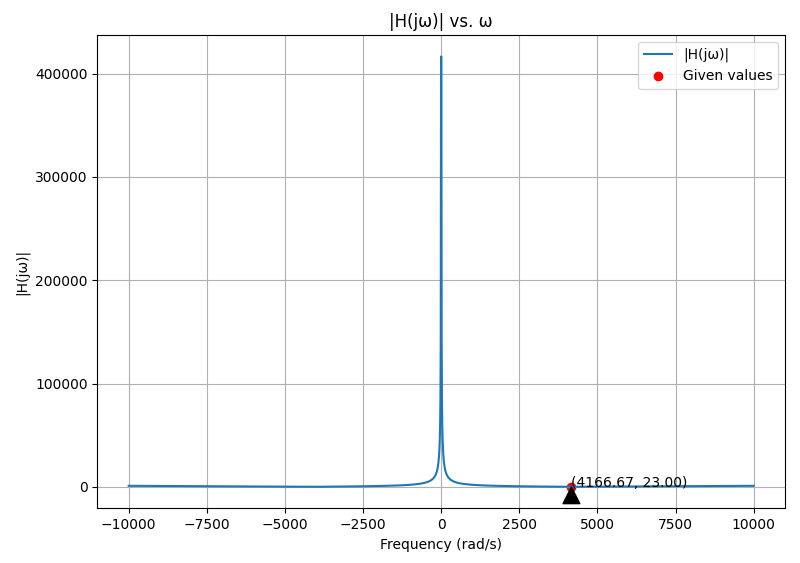
\includegraphics[width=\columnwidth]{figs/analog.png}
  \label{fig:bode_Plot}
  \end{figure}
\end{document}
